\documentclass[draft, twocolumn]{article}
\usepackage[unicode,draft=false,hidelinks]{hyperref}
\usepackage{cite}
\usepackage{catchfilebetweentags}
\usepackage{amssymb}
\usepackage{turnstile}
\usepackage{bbm}
\usepackage[greek, english]{babel}
\usepackage{MnSymbol}
\usepackage{stmaryrd}
\usepackage{csquotes}
\newcommand\doubleplus{+\kern-1.3ex+\kern0.8ex}
\newcommand\mdoubleplus{\ensuremath{\mathbin{+\mkern-8mu+}}}
\makeatletter
\newcommand\incircbin
{%
  \mathpalette\@incircbin
}
\newcommand\@incircbin[2]
{%
  \mathbin%
  {%
    \ooalign{\hidewidth$#1#2$\hidewidth\crcr$#1\bigcirc$}%
  }%
}
\newcommand{\oeq}{\ensuremath{\incircbin{=}}}
\makeatother
\usepackage{ucs}
\DeclareUnicodeCharacter{8759}{\ensuremath{\squaredots}}
\DeclareUnicodeCharacter{951}{\textgreek{\texteta}}
\DeclareUnicodeCharacter{737}{\ensuremath{^\text{l}}}
\DeclareUnicodeCharacter{691}{\ensuremath{^\text{r}}}
\DeclareUnicodeCharacter{7523}{\ensuremath{_\text{r}}}
\DeclareUnicodeCharacter{8718}{\ensuremath{\blacksquare}}
\DeclareUnicodeCharacter{957}{\textgreek{\textnu}}
\DeclareUnicodeCharacter{961}{\textgreek{\textrho}}
\DeclareUnicodeCharacter{929}{\textgreek{\textRho}}
\DeclareUnicodeCharacter{954}{\textgreek{\textkappa}}
\DeclareUnicodeCharacter{10214}{\ensuremath{\lsem}}
\DeclareUnicodeCharacter{10215}{\ensuremath{\rsem}}
\DeclareUnicodeCharacter{8857}{\mdoubleplus}
\DeclareUnicodeCharacter{8860}{\oeq}
\DeclareUnicodeCharacter{9043}{\ensuremath{\triangle}}
\DeclareUnicodeCharacter{928}{\textgreek{\textPi}}
\DeclareUnicodeCharacter{922}{\textgreek{\textKappa}}
\DeclareUnicodeCharacter{931}{\textgreek{\textSigma}}
\DeclareUnicodeCharacter{916}{\textgreek{\textDelta}}
\DeclareUnicodeCharacter{8779}{\ensuremath{\backtriplesim}}
\DeclareUnicodeCharacter{8799}{\ensuremath{\stackrel{?}{=}}}
\DeclareUnicodeCharacter{10181}{\ensuremath{\lbag}}
\DeclareUnicodeCharacter{10182}{\ensuremath{\rbag}}
\usepackage[utf8x]{inputenc}
\usepackage[T1]{fontenc}
\usepackage{autofe}
\usepackage[references]{agda}
\usepackage{bbding}
\setlength{\marginparwidth}{2cm}
\usepackage[obeyDraft]{todonotes}
\usepackage{lineno}
\setlength\linenumbersep{-0.5cm}
\usepackage{amsthm}
\theoremstyle{definition}
\newtheorem{definition}{Definition}[section]
\theoremstyle{remark}
\newtheorem{principle}{Principle}[section]
\usepackage{subcaption}
\usepackage{graphicx}
\usepackage{tikz}
\usetikzlibrary{decorations.pathmorphing}
\usetikzlibrary{snakes}
\usetikzlibrary{arrows}
\usepackage{forest}
\author{D Oisín Kidney}
\title{An Efficient and Flexible Evidence-Providing Polynomial Solver in Agda}
\begin{document}
\maketitle
\begin{abstract}
  We present a new implementation of a ring solver in the programming language
  Agda\cite{norell_dependently_2008}. The new implementation is significantly
  more efficient than the version in the standard
  library\cite{danielsson_agda_2018}, bringing it in line with Coq's \verb+ring+
  tactic\cite{the_coq_development_team_2018_1219885},
  \cite{hutchison_proving_2005}. 

  We demonstrate techniques for constructing proofs based on the theory of
  lists, show how Agda's reflection system can be used to provide a safe and
  simple interface to the solver, and compare the ``correct by construction''
  approach to that of auxiliary proofs.
  
  We also show that, as a by-product of proving equivalences rather than
  equalities, the prover can be used to provide artifacts other than equational
  proofs, including step-by-step solutions, and isomorphisms.
\end{abstract}
\tableofcontents
\section{Introduction}
Dependently typed programming languages allow programmers and mathematicians
alike to write proofs which can be executed. For programmers, this often means
being able to formally verify the properties of their programs; for
mathematicians, it provides a system for writing machine-checked (rather than
hand-checked) proofs.

Naïve usage of these systems can be tedious: the typechecker is often
over-zealous in its rigor, demanding justification for every minute step in a
proof, no matter how obvious or trivial it may seem to a human. For algebraic
proofs, this kind of thing usually consists of long chains of rewrites, of the
style ``apply commutativity of \(+\), then associativity of \(+\), then at this
position apply distributivity of \(*\) over \(+\)'' and so on, when really the
programmer wants to say ``rearrange the expression into this form, checking it's
correct''.

However, since our proof assistant is also a programming language, we can
automate this process by writing a verified program to compute these proofs for
us. 
\section{A Case Study in Monoids}
Before describing the ring solver, first we will explain the technique of
writing a solver in Agda in the simpler setting of monoids.

\begin{definition}{Monoids}
  A monoid is a set equipped with a binary operation, \(\bullet\), and a
  distinguished element \(\epsilon\), such that the following equations hold:
  \begin{align}
    x \bullet (y \bullet z) &= (x \bullet y) \bullet z \tag{Associativity} \\
    x \bullet \epsilon      &= x \tag{Left Identity} \\
    \epsilon \bullet x      &= x \tag{Right Identity}
  \end{align}
\end{definition}
Addition and multiplication (with 0 and 1 being the respective identity
elements) are perhaps the most obvious instances of the algebra. In computer
science, monoids have proved a useful abstraction for formalizing concurrency
(in a sense, an associative operator is one which can be evaluated in any
order).

Monoids can be represented in Agda in a straightforward way, as a record (see
Figure~\ref{mon-def}). Immediately it should be noted that we're no longer
talking about a monoid over a set, but rather one over a setoid. In other words,
rather than using propositional equality (indicated by the \(\AgdaDatatype{≡}\)
symbol), we will use a user-supplied equivalence relation (\(\AgdaField{≈}\) in
Figure~\ref{mon-def}) in our proofs.
\begin{figure}
  \ExecuteMetaData[Monoids.tex]{mon-def}
  \caption{The definition of Monoid in the Agda Standard
    Library\cite{danielsson_agda_2018}}
  \label{mon-def}
\end{figure}
\subsection{Equivalence Proofs}
Propositions are stated in type signatures in dependently typed languages.
Figure~\ref{mon-ident} is an example of such a proposition.
\begin{figure}[h]
  \ExecuteMetaData[Monoids.tex]{mon-ident}
  \caption{Example Identity}
  \label{mon-ident}
\end{figure}
To a human, the fact that the identity holds may well be obvious:
\(\AgdaField{∙}\) is associative, so we can scrub out all the parentheses, and
\(\AgdaField{ε}\) is the identity element, so scrub it out too. After that, both
sides are equal, so voilà!

Unfortunately, to convince the compiler we need to specify every instance of
associativity and identity, rewriting the left-hand-side repeatedly until it
matches the right:

\begin{samepage}
  \begin{linenumbers}
    \ExecuteMetaData[Monoids.tex]{mon-proof}
  \end{linenumbers}
\end{samepage}

The syntax is designed to mimic that of a handwritten proof: line 3 is the
expression on the left-hand side of \(\AgdaField{≈}\) in the type, and line 9
the right-hand-side. In between, the expression is repeatedly rewritten into
equivalent forms, with justification provided inside the angle brackets. For
instance, to translate the expression from the form on line 3 to that on line 5,
the associative property of \(\AgdaField{∙}\) is used on line 4.

Because we're not using propositional equality, some familiar tools are
unavailable, like Agda's rewrite mechanism, or function congruence (this is why
we have to explicitly specify the congruence we're using on line 6). The purpose
of this particular hair shirt is flexibility: users can still use the solver
even if their type only satisfies the monoid laws modulo some equivalence
relation (perhaps they are have an implementation of finite, mergeable sets as
balanced trees, and want to treat two sets as equivalent if their elements are
equal, even if their internal structures are not). Beyond flexibility, we get
some other interesting applications, which are explored in
section~\ref{setoid-applications}.

Despite the pleasant syntax, the proof is mechanical, and it's clear that
similar proofs would become tedious with more variables or more complex algebras
(like rings). To avoid the tedium, then, we automate the procedure.
\subsection{Canonical Forms}
Automation of equality proofs like the one above can be accomplished by first
rewriting both sides of the equation into a canonical form. Not every algebra
has a canonical form: monoids do, though, and it's the simple list.
\ExecuteMetaData[Monoids.tex]{list-def}
We're going to treat this type like an AST for a simple ``language of lists''.
This language supports two functions: the empty list, and concatenation.
\ExecuteMetaData[Monoids.tex]{list-monoid}
The type itself parameterized by the number of variables it contains. Users can
refer to variables by their index:
\ExecuteMetaData[Monoids.tex]{list-vars}
And we can interpret this language with values for each variable supplied in a
vector:
\ExecuteMetaData[Monoids.tex]{list-eval}

Compare this language to the language of monoid expressions that
Figure~\ref{mon-ident} uses: both have identity elements and a binary operator,
and both refer to variables. Our language of lists, however, has one significant
advantage: the monoid operations don't depend on the contents of the lists, only
the structure. In other words, an expression in the language of lists will
reduce to a flat list even if it has elements which are abstract variables. As a
result, the identity from Figure~\ref{mon-ident} is \emph{definitionally} true
when written in the language of lists:
\ExecuteMetaData[Monoids.tex]{list-obvious}
\subsection{Extracting Evidence}
While this is beginning to look like a solver, it's still not entirely clear how
we're going to join up the pieces. The first step is to get a concrete
representation of expressions which we can manipulate and pattern-match on
(Figure~\ref{mon-ast}).
\begin{figure}[h]
  \ExecuteMetaData[Monoids.tex]{mon-ast}
  \caption{The AST for monoid expressions}
  \label{mon-ast}
\end{figure}
It has constructors for each of the monoid operations
(\(\AgdaInductiveConstructor{⊕}\) and \(\AgdaInductiveConstructor{e}\) are
\(\AgdaField{∙}\) and \(\AgdaField{ε}\), respectively), and it's indexed by the
number of variables it contains, which are constructed with
\(\AgdaInductiveConstructor{ν}\).

We can convert from this AST to an unnormalized expression like so\footnotemark:
\ExecuteMetaData[Monoids.tex]{eval-ast}
Because this function performs no normalization or transformation, the output is
definitionally equal to its equivalent expression. This means that we can
discharge the proof obligation with \(\AgdaFunction{refl}\):
\footnotetext{
  The type of the unnormalized expression has changed slightly: instead of being
  a curried function of \(n\) arguments, it's now a function which takes a
  vector of length \(n\). The final solver has an extra translation step for
  going between these two representations, but it's a little fiddly, and not
  directly relevant to what we're doing here, so we've glossed over it. We refer
  the interested reader to the Relation.Binary.Reflection module of Agda's
  standard library\cite{danielsson_agda_2018} for an implementation.
}
\ExecuteMetaData[Monoids.tex]{eval-nonnorm}

The AST might look ugly, but it gives us a link between the expressions we had
in Figure~\ref{mon-ident} and a concrete representation. The next link is
between the AST and the normalized expression. We can convert from the AST to a
normal form like so:
\ExecuteMetaData[Monoids.tex]{ast-norm}
And since we already defined how to ``evaluate'' the list normal form, we can
combine both steps into one:
\ExecuteMetaData[Monoids.tex]{ast-norm-interp}

Now we have a concrete way to link the normalized and non-normalized forms of
the expressions. A diagram of the strategy for constructing our proof is in
Figure~\ref{proof-process}. The goal is to construct a proof of equivalence
between the two expressions at the bottom: to do this, we first construct the
AST which represents the two expressions (for now, we'll assume the user
constructs this AST themselves. Later we'll see how too construct it
automatically from the provided expressions). Then, we can evaluate it into
either the normalized form, or the unnormalized form. Since the normalized forms
are syntactically equal, all we need is \(\AgdaInductiveConstructor{refl}\) to
prove their equality. The only missing part now is \(\AgdaFunction{correct}\),
which is the task of the next section.

\begin{figure*}
  \makebox[\textwidth][c]{
    \begin{tikzpicture}
      % \draw[help lines] (-8,-4) grid (8,3); 
      \node (ln) at (-2, 2) {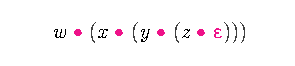
\includegraphics[draft=false,trim={25 10 25 10}]{graphics/rhs-norm}};
      \node (rn) at ( 2, 2) {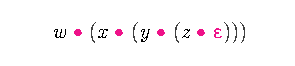
\includegraphics[draft=false,trim={25 10 25 10}]{graphics/rhs-norm}};
      \node (la) at (-6, 0) {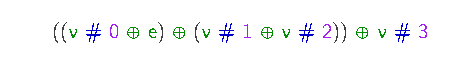
\includegraphics[draft=false,trim={25 10 22 10}]{graphics/lhs-ast}};
      \node (ra) at ( 6, 0) {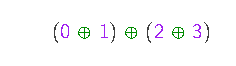
\includegraphics[draft=false,trim={25 10 48 10}]{graphics/rhs-ast}};
      \node (le) at (-2,-2) {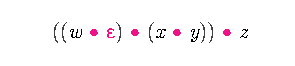
\includegraphics[draft=false,trim={25 10 23 10}]{graphics/lhs-expr}};
      \node (re) at ( 2,-2) {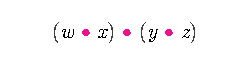
\includegraphics[draft=false,trim={25 10 20 10}]{graphics/rhs-expr}};
      \draw[|-stealth] (la) to[out=90 , in=180] node[midway, fill=white] {\AgdaFunction{⟦\_⇓⟧}} (ln);
      \draw[|-stealth] (la) to[out=270, in=180] node[midway, fill=white] {\AgdaFunction{⟦\_⟧} } (le);
      \draw[|-stealth] (ra) to[out=90 , in=0  ] node[midway, fill=white] {\AgdaFunction{⟦\_⇓⟧}} (rn);
      \draw[|-stealth] (ra) to[out=270, in=0  ] node[midway, fill=white] {\AgdaFunction{⟦\_⟧} } (re);
      \foreach \e/\n in {le/ln,re/rn}
        \foreach \shft in {-0.6pt,0.6pt}
          \draw[AgdaField, transform canvas={xshift=\shft}, snake=coil, segment aspect=0, segment amplitude=0.4pt, segment length=4pt] (\e) -- (\n);
      \node[fill=white] at (-2, 0) {\AgdaFunction{correct}};
      \node[fill=white] at ( 2, 0) {\AgdaFunction{correct}};
      \foreach \shft in {-1.6pt, 0pt}
        \draw[AgdaDatatype, transform canvas={yshift=\shft}] (ln) -- (rn);
      \draw[AgdaDatatype, transform canvas={yshift=1.6pt}] (ln) -- (rn) node[midway, above] {\AgdaInductiveConstructor{refl}};
      \draw[-angle 90, dashed] (re) to[out=270, in=270] node[near start, fill=white] {\AgdaKeyword{quoteTerm}} ([shift={(1,0)}]ra.south);
      \draw[-angle 90, dashed] (le) to[out=270, in=270] node[near start, fill=white] {\AgdaKeyword{quoteTerm}} ([shift={(-1,0)}]la.south);
    \end{tikzpicture}
  }
  \caption{The Reflexive Proof Process}
  \label{proof-process}
\end{figure*}
\todo{
  equivalent diagram for correct by construction
  (section~\ref{correct-by-constr})
}

\subsection{Homomorphism}

Taking the non-normalizing interpreter as a template, the three cases are as
follows\footnotemark:
\begin{align}
  \AgdaFunction{⟦} x \AgdaInductiveConstructor{⊕} y \AgdaFunction{⟧} \rho \;
    &\AgdaField{≈} \; \AgdaFunction{⟦} x \AgdaInductiveConstructor{⊕} y
    \AgdaFunction{⇓⟧} \rho \label{plus-hom} \\
  \AgdaFunction{⟦} \AgdaInductiveConstructor{e} \AgdaFunction{⟧} \rho \;
    &\AgdaField{≈} \; \AgdaFunction{⟦} \AgdaInductiveConstructor{e}
    \AgdaFunction{⇓⟧} \rho \label{e-hom} \\
  \AgdaFunction{⟦} \AgdaInductiveConstructor{ν} i \AgdaFunction{⟧} \rho \;
    &\AgdaField{≈} \; \AgdaFunction{⟦} \AgdaInductiveConstructor{ν} i
    \AgdaFunction{⇓⟧} \rho \label{var-hom}
\end{align}
\footnotetext{
  Equations \ref{plus-hom} and \ref{e-hom} comprise a monoid
  homomorphism.
}

Proving each of these cases in turn finally verifies the correctness of our list
language.
\ExecuteMetaData[Monoids.tex]{correct-ast}

\subsection{Usage}
Combining all of the components above, with some plumbing provided by the
\(\AgdaModule{Relation.Binary.Reflection}\) module, we can finally automate the
solving of the original identity in figure~\ref{mon-ident}:
\ExecuteMetaData[Monoids.tex]{ident-auto-proof}

\section{A Polynomial Solver}
We now know the components required for an automatic solver for some algebra: a
canonical form, a concrete representation of expressions, and a proof of
correctness. We now turn our focus to polynomials.

Prior work in this area includes\cite{geuvers_automatically_2017},
\cite{meshveliani_dependent_2013}, \cite{zalakain_evidence-providing_2017},
\cite{cheng_functional_2018}, and \cite{russino_polynomial_2017}, but perhaps
the state-of-the-art (at least in terms of efficiency) is Coq's \texttt{ring}
tactic\cite{the_coq_development_team_2018_1219885}, which is based on an
implementation described in\cite{hutchison_proving_2005}.
\subsection{Choice of Algebra}
The choice of algebra has been glossed over thus far, but it is an important
design decision: choose one with too many laws, and the solver becomes unusable
for several types; too few, and we may miss out on normalization opportunities.

The algebra defined in \cite{hutchison_proving_2005} is that of an
\emph{almost-ring}. It's very close in definition too a ring, but it discards
the requirement that negation is an inverse (\(x + (-x) = 0\)). Instead, it
merely requires that negation distribute over addition and multiplication
appropriately. This allows the solver to be used with non-negative types, like
\(\mathbb{N}\), where negation is simply the identity function.

A potential worry is that because we don't require \(x + (-x) = 0\)
axiomatically, it won't be provable in our system. This is not so: as long as
\(1 - 1\) reduces to \(0\) in the coefficient set, the solver will verify the
identity.
\section{Horner Normal Form}
The canonical representation of polynomials is a list of coefficients, least
significant first (``Horner Normal Form''). Our initial attempt at encoding this
representation will begin like so:
\ExecuteMetaData[Rings.tex]{dense-opening}

The entire module is parameterized by the choice of coefficient. This
coefficient should support the ring operations, but it is ``raw'', i.e. it
doesn't prove the ring laws. The operations on the polynomial itself are defined
like so\footnotemark:
\ExecuteMetaData[Rings.tex]{dense-impl}
\footnotetext{
  Symbols chosen for operators use the following mnemonic:
  \begin{enumerate}
    \item Operators preceded with ``\(\mathbb{N}.\)'' are defined over
      \(\mathbb{N}\); e.g. \(\mathbb{N}.+\), \(\mathbb{N}.*\).
    \item Plain operators, like \(+\) and \(*\), are defined over the
      coefficients.
    \item Boxed operators, like \(\boxplus\) and \(\boxtimes\), are defined over
      polynomials.
    \item Operators which are boxed on one side are defined over polynomials on
      the corresponding side, and the coefficient on the other; e.g.
      \(\ltimes\), \(\rtimes\).
  \end{enumerate}
}

Finally, evaluation of the polynomial uses ``Horner's rule'' to minimize
multiplications:
\ExecuteMetaData[Rings.tex]{dense-eval}
\subsection{Sparse Horner Normal Form}
As it stands, the above representation has two problems:

\begin{description}
  \item[Redundancy] The representation suffers from the problem of trailing
    zeroes. In other words, the polynomial $2x$ could be represented by any of
    the following:
  
    \begin{align*}
      & 0, 2 \\
      & 0, 2, 0 \\
      & 0, 2, 0, 0 \\
      & 0, 2, 0, 0, 0, 0, 0
    \end{align*}
    
    This is a problem for a solver: the whole \emph{point} is that equivalent
    expressions are represented the same way.

  \item[Inefficiency] Expressions will tend to have large gaps, full only of
    zeroes. Something like $x^5$ will be represented as a list with 6 elements,
    only the last one being of interest. Since addition is linear in the length
    of the list, and multiplication quadratic, this is a major concern.
\end{description}

In\cite{hutchison_proving_2005}, the problem is addressed primarily from the
efficiency perspective: they add a field for the ``power index''. For our case,
we'll just store a list of pairs, where the second element of the pair is the
power index\footnote{
  In\cite{hutchison_proving_2005}, the expression \((c , i) \squaredots P\)
  represents \(P \times X^i + c\). We found that \(X^i \times (c + X \times P)\)
  is a more natural translation, and it's what we use here. A power index of
  \(i\) in this representation is equivalent to a power index of \(i+1\)
  in\cite{hutchison_proving_2005}.
}.

As an example, the polynomial:
\[ 3 + 2x^2 + 4x^5 + 2x^7 \]
Will be represented as:
\[ (3,0),(2,1),(4,2),(2,1) \]
Or, mathematically:
\[ x^0 (3 + x x^1 (2 + x x^2 * (4 + x x^1 (2 + x 0)))) \]

\begin{definition}{Dense and Sparse Encodings.}
  In situations like this, where inductive types have large ``gaps'' of
  zero-like terms between interesting (non-zero-like) terms, the encoding which
  uses an index to represent the distance to the next interesting term will be
  called \emph{sparse}, and the encoding which simply stores the zero term will
  be called \emph{dense}.
\end{definition}
\subsubsection{Uniqueness}
While this form solves our efficiency problem, we still have redundant
representations of the same polynomials. In\cite{hutchison_proving_2005}, care
is taken to ensure all operations include a normalizing step, but this is not
verified: in other words, it is not proven that the polynomials are always in
normal form.

Expressing that a polynomial is in normal form turns out to be as simple as
disallowing zeroes: without them, there can be no trailing zeroes, and all gaps
must be represented by power indices. To check for zero, we require the user
supply a decidable predicate on the coefficients. This changes the module
declaration like so:
\ExecuteMetaData[Rings.tex]{sparse-opening}

Finally, we can define a sparse encoding of Horner Normal Form:
\ExecuteMetaData[Rings.tex]{sparse-decl}

The proof of nonzero is marked irrelevant (preceded with a dot) to avoid
computing it at runtime.

We can wrap up the implementation with a cleaner interface by providing a
normalizing version of \(\AgdaInductiveConstructor{\_∷\_}\):
\ExecuteMetaData[Rings.tex]{sparse-norm}
\subsubsection{Comparison}
Our addition and multiplication functions will need to properly deal with the
new sparse formulation. First things first, we'll need a way to match the power
indices. We can use a function from\cite{mcbride_view_2004} to do so.
\ExecuteMetaData[Rings.tex]{compare}
This is a classic example of a ``leftist'' function: after pattern matching on
one of the constructors of \(\AgdaDatatype{Ordering}\), it gives you information
on type variables to the \emph{left} of the pattern. In other words, when you
run the function on some variables, the result of the function will give you
information on its arguments.
\subsubsection{Efficiency}
The implementation of \(\AgdaFunction{compare}\) may raise suspicion with
regards to efficiency: if this encoding of polynomials improves time complexity
by skipping the gaps, don't we lose all of that when we encode the gaps as Peano
numbers?

The answer is a tentative no. Firstly, since we are comparing gaps, the
complexity can be no larger than that of the dense implementation. Secondly, the
operations we're most concerned about are those on the underlying coefficient;
and, indeed, this sparse encoding does reduce the number of those significantly.
Thirdly, if a fast implementation of \(\AgdaFunction{compare}\) is really and
truly demanded, there are tricks we can employ.

Agda has a number of built-in functions on the natural numbers: when applied to
closed terms, these call to an implementation on Haskell's \texttt{Integer}
type, rather than the unary implementation. For our uses, the functions of
interest are \(\AgdaFunction{-}\), \(\AgdaFunction{+}\), \(\AgdaFunction{<}\),
and \(\AgdaFunction{==}\). The comparison functions provide booleans rather than
evidence, but we can prove they correspond to the evidence-providing versions.
Combined with judicious use of \(\AgdaFunction{erase}\), we get the following:
\ExecuteMetaData[Rings.tex]{unsafe-compare}
\subsubsection{Termination}
Unfortunately, using \(\AgdaFunction{compare}\) in the most obvious way won't
pass the termination checker.
\ExecuteMetaData[Rings.tex]{nonterminating-addition}

Agda needs to be able to see that one of the numbers returned by
\(\AgdaFunction{compare}\) always reduces in size: however, since the difference
is immediately packed up in a list in the recursive call, it's buried too deeply
in constructors for the termination checker to see it.

\begin{principle}{To make termination obvious, perform call pattern
    specialization.}
The solution is twofold: unpack any constructors into function arguments as soon
as possible, and eliminate any redundant pattern matches in the offending
functions. Taken together, these form an transformation known as ``call pattern
specialization''\cite{jones_call-pattern_2007}\footnotemark. Happily, this
transformation both makes termination more obvious \emph{and} improves
performance.
\end{principle}

\footnotetext{
  This transformation is performed automatically by GHC as an optimization:
  perhaps a similar transformation could be performed by Agda's termination
  checker to reveal more terminating programs.
}

\begin{figure}[h]
  \ExecuteMetaData[Rings.tex]{addition}
  \caption{Terminating Addition, Using Call-Pattern Specialization}
  \label{mono-addition}
\end{figure}
Every helper function in the mutual block matches on exactly one argument,
eliminating redundancy. This also simplifies some of the homomorphism proofs
later on.

\todo{
  You can probably get the foldr version of these functions to pass the
  termination checker if you use a sized type.
  \cite{abel_miniagda_2010}
  \cite{allais_three_2016}
}
\section{Binary}
Before continuing with polynomials, we'll take a short detour to look at binary
numbers. These have a number of uses in dependently typed programming: as well
as being a more efficient alternative to Peano numbers, their structure informs
that of many data structures, such as binomial heaps, and as such they're used
in proofs about those structures.

Similarly to polynomials, though, the naïve representation suffers from
redundancy in the form of trailing zeroes. There are a number of ways to
overcome this (see\cite{meshveliani_binary-4_2018}
and\cite{escardo_libraries_2018}, for example); yet another is the repurposing
of our sparse polynomial from above.
\ExecuteMetaData[Binary.tex]{binary-def}
We don't need to store any coefficients, because 1 is the only permitted
coefficient. Effectively, all we store is the distance to another 1.

Addition (elided here for brevity) is linear in the number of bits, as expected,
and multiplication takes full advantage of the sparse representation:
\ExecuteMetaData[Binary.tex]{binary-mul}
\section{Multivariate}
Up until now our polynomial has been an expression in just one variable. For it
to be truly useful, though, we'd like to be able to extend it to many: luckily
there's a well-known isomorphism we can use to extend our earlier
implementation. For a polynomial with two variables, we will represent it as a
polynomial whose coefficients are themselves polynomials of one variable. For
three, it'll be a polynomial whose coefficients are polynomials in two
variables, and so on. Generally speaking, a multivariate polynomial is one where
its coefficients are polynomials with one fewer
variable\cite{cheng_functional_2018}.

Before jumping to implement this, though, we should notice an opportunity for
optimization (also pointed out in\cite{hutchison_proving_2005}). Just like how
the monomials had gaps of zeroes between non-zero terms, this type will have
gaps of constant polynomials between non-constant polynomials. In other words,
in a expression of \(n\) variables, information about the last variable will be
hidden behind \(n\) layers of nesting. If those \(n\) layers don't contain any
information (i.e. they're all constant), we want to skip all that nesting with
an \emph{injection} index (like the power index).
\subsection{Sparse Nesting}
It's immediately clear that removing the gaps from the nesting will be more
difficult than it was for the exponents: the \(\AgdaDatatype{Poly}\) type is
\emph{indexed} by the number of variables it contains, so any manipulation of
the injection index will have to correspond carefully to the
\(\AgdaDatatype{Poly}\)'s index.

Our first approach might mimic the structure of \(\AgdaDatatype{Ordering}\),
with an indexed type:
\ExecuteMetaData[Poly.tex]{poly-slime}
Where \(\AgdaDatatype{FlatPoly}\) is effectively the gappy type we had earlier.
If you actually tried to use this type, though, you'd run into issues: because
it's an indexed type, pattern matching on it will force unification of the index
with whatever type variable it was bound to. This is problematic because the
index is defined by a function: pattern match on a pair of
\(\AgdaDatatype{Poly}\)s and you're asking Agda to unify \(i_1 + j_1\) and
\(i_2 + j_2\), a task it will likely find too difficult. How do we avoid this?
``Don't touch the green slime!''\cite{mcbride_polynomial_2018}:
\begin{displayquote}
  When combining prescriptive and descriptive indices, ensure both are in
  constructor form. Exclude defined functions which yield difficult unification
  problems.
\end{displayquote}
We'll have to take another route.
\subsubsection{Inequalities}
First, we'll define our polynomial like so:
\ExecuteMetaData[Poly.tex]{poly}
The type is now parameterized, rather than indexed: our pattern-matching woes
have been solved. Also, the gap is now implicit; instead, we store a proof that
the nested polynomial has no more variables then the outer. Next,
\(\AgdaDatatype{FlatPoly}\):
\ExecuteMetaData[Poly.tex]{flat-poly}
We're back to an indexed type here, so you may be concerned about similar
unification problems like the ones we had above: not to worry, though, as these
indices are in constructor form, which prove much easier to unify than
functions.

Also new here is the \(\AgdaFunction{Norm}\) function. It serves the same
purpose that \(\AgdaFunction{Zero}\) did in the monomial, ensuring that there
are no constant polynomials which could be replaced by incrementing the
injection index. Its definition is as follows:
\ExecuteMetaData[Poly.tex]{poly-norm}

The rest of types are similar to what they were before:
\ExecuteMetaData[Poly.tex]{poly-types}
Again, similarly to the sparse exponent encoding, we provide a smart
constructor which ensures normalization.
\subsubsection{Choosing an Inequality}
Conspicuously missing above is a definition for \(\leq\). This choice has
important performance implications, and exploring the various design avenues
turned out to be more difficult than anticipated. As a jumping-off point, we'll
look at the three definitions of \(\leq\) in the Agda standard
library\cite{danielsson_agda_2018}.
\begin{description}
  \item[Option 1: The Standard Way] The most commonly used definition of
    \(\leq\) is as follows:
    \ExecuteMetaData[Poly.tex]{leq-1}
    Trying to proceed with this type will yield a nasty performance bug, though:
    first, remember the functions defined on the sparse exponent encoding above.
    When dealing with two polynomials, they'll have to line them up, comparing
    the respective gaps to find where two coefficients coincide (see
    \(\AgdaFunction{⊞-zip}\) in figure~\ref{mono-addition}). We'll have to do
    the same with this version of sparseness: however, since we're no longer
    storing the gaps, the comparison will be on the size of the nested
    polynomial. To see why this is a problem, consider the following sequence of
    nestings:

    \[ (5 ≤ 6), (4 ≤ 5), (3 ≤ 4), (1 ≤ 3), (0 ≤ 1) \]

    The outer polynomial has 6 variables, but it has a gap to its inner
    polynomial of 5, and so on. The comparisons will be made on 5, 4, 3, 1, and
    0. Like repeatedly taking the length of the tail of a list, this is
    quadratic. There must be a better way.
  \item[Option 2: With Propositional Equality] Once you realize we need to be
    comparing the gaps and not the tails, another encoding of \(\leq\) in
    Data.Nat seems the best option:
    \ExecuteMetaData[Poly.tex]{leq-2}
    It stores the gap \emph{right there}: in \(\AgdaField{k}\)!

    Unfortunately, though, we're still stuck. While you can indeed run your
    comparison on \(k\), you're not left with much information about the rest.
    Say, for instance, you find out that two respective \(\AgdaField{k}\)s are
    equal. What about the \(m\)s? Of course, you \emph{can} show that they must
    be equal as well, but it requires a proof. Similarly in the less-than or
    greater-than cases: each time, you need to show that the information about
    \(\AgdaField{k}\) corresponds to information about \(m\). Again, all of this
    can be done, but it all requires propositional proofs, which are messy, and
    slow. Erasure is an option, but I'm not sure of the correctness of that
    approach.
  \item[Option 3] What we really want is to \emph{run} the comparison function
    on the gap, but get the result on the tail. Turns out we can do exactly that
    with the following:
    \ExecuteMetaData[Poly.tex]{leq-3}
    While this structure stores the inequality by induction on the gap.
\end{description}
As long as the comparison uses the inductive structure of the final definition
of \(\leq\) above, it will have the correct complexity, while providing the
comparison result about the correct type variables. With a slightly different
definition of \(\AgdaDatatype{Ordering}\), we get the following:
\ExecuteMetaData[Poly.tex]{leq-3-cmp}

A few things to note here:
\begin{itemize}
  \item The \(\AgdaFunction{≤-compare}\) function is one of those reassuring
    ones which Agda can completely infer.
 \item This function looks somewhat similar to the normal definition of
   \(\AgdaFunction{compare}\) and as a result, the ``matching'' logic for degree
   and number of variables began too look similar.
\end{itemize}
\subsubsection{Axiom K}
With this approach, we can indeed write all of the functions we need, but we
will run into trouble trying to prove homomorphism.

The issue revolves around the fact that \(\leq\) is \emph{irrelevant}. In other
words, if you have two proofs of (say) \(n \leq m\), then those two proofs must
also be propositionally equal. When we're trying to prove that two polynomials
evaluate to the same thing, we'd like to rely on this property.

Unfortunately, though, proving this without axiom K is difficult. However, we
should notice that we didn't need to prove anything like this when dealing with
the sparse exponent encoding: why do we have to now?

\subsubsection{Indexed Ordering}
The issue lies in our newer definition of \(\AgdaDatatype{Ordering}\): whereas
the standard definition (on \(\AgdaDatatype{ℕ}\)) provided information about the
arguments to the comparison function, the new definition provides only
information about their \emph{indices}. When pattern matching on the result of
the comparison before, we got all the equality information we needed about the
\(\leq\) proofs.

To solve the problem, we'll more closely mimic the old comparison, and provide a
result on the \(\leq\) proofs directly. We should first look for an equivalent
to addition. This turns out to be transitivity:
\ExecuteMetaData[Poly.tex]{trans}

With this defined, the \(\AgdaDatatype{Ordering}\) type is obvious:
\ExecuteMetaData[Poly.tex]{ind-ordering}
\subsection{Operations}
After adding the injection index optimization, we use a normalizing version of
\(\AgdaInductiveConstructor{Π}\), like we did for the power indices
(Figure~\ref{norm-nest}). Operations now perform two ``match-up'' operations:
one for the injection indices and one for the power indices
(Figure~\ref{full-mul}). \todo{Maybe unify the two match-up functions?}

\subsubsection{Termination, Again}
Unfortunately, by introducing gaps into the encoding of nested polynomials, we
have obscured the fact that the recursive call into the nested polynomial is
safe (i.e. it strictly decreases in size). As a result, our functions are no
longer obviously terminating:
\ExecuteMetaData[Poly.tex]{nonterminating-negation}

There are a number of ways to deal with the problem. First, we can remove the
use of a higher-order function:
\ExecuteMetaData[Poly.tex]{no-higher-order}

Agda can track termination through mutual functions: what we've done here is
exposed the fact that the argument passed to \(\AgdaFunction{⊟}\) was embedded
in a constructor of the original type recursed on, meaning it's strictly
smaller. Calling \(\AgdaFunction{foldr}\) breaks this link, and therefore
doesn't pass the termination checker.

However, we would like to use higher-order functions, especially in the more
complex functions like \(\AgdaFunction{⊞}\) and \(\AgdaFunction{⊠}\). There are
a number of techniques to solve the problem, which we'll go through here.

\paragraph{Sized Types}
The Agda compiler recently included a notion of ``size'' for its
types\cite{abel_miniagda_2010}. To demonstrate this, we'll first start with a
standard definition of a rose tree:
\ExecuteMetaData[Rose.tex]{rose}
Level-wise enumeration (Figure~\ref{levelorder}) is an example of a function
with a non-obvious termination pattern:
\ExecuteMetaData[Rose.tex]{nonterminating-rose}

\begin{figure}
  \centering
  \begin{forest}
    [ 1
      [ 2
        [ 9 ]
        [ 10 [11] ]
      ]
      [ 3
        [ 5 ]
      ]
      [ 4
        [ 6
          [ 7 ]
          [ 8 ]
        ]
      ]
    ]
  \end{forest}
  \[[[1], [2,3,4],[9,10,5,6],[11,7,8]]\]
  \caption{Level-Order Traversal of a Tree}
  \label{levelorder}
\end{figure}

Again, the problem could be solved by avoiding the higher-order
\(\AgdaFunction{foldr}\):
\ExecuteMetaData[Rose.tex]{terminating-rose}

But now we have a far inferior function, and we can't reuse code about lists.

A solution is to add a \emph{size} parameter to the rose tree:
\ExecuteMetaData[Rose.tex]{sized-rose}

The size parameter functions like \(\AgdaDatatype{ℕ}\) might for termination: if
we track it in the recursive calls, it's evidence for decreasing size.
\ExecuteMetaData[Rose.tex]{sized-rose-levels}

You'll notice that the top-level function doesn't specify the size it takes: it
defaults to \(\infty\), only being used where you need it for termination.

Unfortunately for us, this approach won't work: remember that we normalize the
nesting of polynomials (Figure~\ref{norm-nest}). This means we may remove one
layer of nesting on certain polynomials, which would mean a change in the size
parameter itself. This means we can't use the nice signature that the level-wise
traversal has above: we'd need something a little more involved. What we
\emph{do} know is that the internal poly always has a \emph{smaller} size than
the external, but here we must stop, recognizing that we're about to duplicate
the logic we already encoded with the \(\leq\) proofs. Luckily for us, there
\emph{is} a way to use these to give us what we want.

\begin{figure*}
  \centering
  \ExecuteMetaData[Poly.tex]{poly-norm-inj}
  \caption{Normalizing Nesting}
  \label{norm-nest}
\end{figure*}

\paragraph{Well-Founded Recursion}
Among the bag of tricks available to Agda programmers to prove termination is
what's known as \emph{well-founded recursion}\cite{nordstrom_terminating_1987}.
It works by providing a relation which describes some strictly decreasing finite
chain: \(<\) on \(\mathbb{N}\), for instance. It's strictly decreasing (the
first argument always gets smaller, in contrast to, say, \(\leq\)), and it's
finite, because it must end at 0.

It's a powerful tool, which can be used to prove complex termination patterns:
multiple relations can be combined lexicographically, for instance, if the
recursive function decreases on different arguments in different settings.

In Agda,  well-founded recursion is specified with the following type:
\ExecuteMetaData[Poly.tex]{acc-def}

This type is a way to construct arguments to functions which are strictly
decreasing in size. Simply add it as an extra parameter to the dangerous
functions, pattern match on \(\AgdaInductiveConstructor{acc}\), and you've
provided evidence that an argument is strictly decreasing.

One of the warts of well-founded recursion is that usually the programmer has to
separately construct the relation they're interested in. As well as being
complex, it can be computationally expensive to do so. Usually the compiler can
elide the calls, recognizing that the argument isn't used, but the optimization
can't be guaranteed.

Luckily, in our case, the relation is already lying around, in the injection
index. So we can just use that!
\ExecuteMetaData[Poly.tex]{with-acc}

\subsection{Semantics}
When it comes to ``interpreting'' the polynomials, we don't need to use the same
ring as we did for the coefficients: all we need is a homomorphism between the
coefficients and the target. This allows the user to supply (potentially) a more
efficient implementation for the coefficients, and then use it to prove things
about some slower target type. The declaration for the semantics module, then,
looks like this:
\ExecuteMetaData[Poly.tex]{semantics-opening}

Finally, for the interpretation functions, we see again evidence that our
choice of inequality was the right one: it naturally works with the vector
input, dropping elements in linear time.
\ExecuteMetaData[Poly.tex]{semantics}

\section{Writing The Proofs}
The proofs are long (roughly 1000 lines), albeit mechanical. There are some
techniques that made the size manageable.
\subsection{Equational Reasoning Techniques}
\subsubsection{Operators}
Because congruence has to be explicitly stated in the reasoning tools, quite
often you'll find yourself writing long chains of \(\AgdaFunction{+-cong}\) or
\(\AgdaFunction{*-cong}\) just to focus into one expression buried in a larger
one. To that end, we can use the following operators to make the ``focusing''
code shooter and easier to read:
\ExecuteMetaData[Reasoning.tex]{cong-combinators}

Their fixty means that they can be chained without parentheses. Something like: 
``\(\AgdaFunction{≪+}\) \(\AgdaFunction{*≫}\) \(\AgdaFunction{*≫}\)
\(\AgdaFunction{≪*}\)'' means ``go to the left of \(+\), then
to the right of \(*\), right again, then to the left of \(*\)''. In other words,
it can take a proof of \(x \; \AgdaField{≈} \; y\), and put it in a larger
context:
\ExecuteMetaData[Reasoning.tex]{cong-example}

\subsubsection{Examples}
\todo{Expand on the proofs. Maybe include an example proof?}
\subsection{The Algebra of Programming and List Homomorphisms}

The algebra of programming\cite{bird_algebra_1997} has been adapted to the
dependently typed setting\cite{mu_algebra_2009}. Along with Horner's
rule\cite{gibbons_horners_2011}, we use it here in the construction of proofs.
First, a relational fold:\todo{This actually works, but needs to be expanded upon.}
\ExecuteMetaData[Poly.tex]{aopa}

\section{Reflection} \label{reflection}
One annoyance of the automated solver is that we have to write the expression we
want to solve twice: once in the type signature, and again in the argument
supplied to solve. Agda can infer the type signature:
\ExecuteMetaData[Monoids.tex]{ident-infer-proof}
But we would prefer to write the expression in the type signature, and have it
infer the argument to solve, as the expression in the type signature is the
desired equality, and the argument to solve is something of an implementation
detail.

This inference can be accomplished using Agda's reflection
mechanisms\cite{van_der_walt_reflection_2012}.

Reflection in Agda allows a program to inspect and modify its own code. Here, it
will allow us to build the AST representation of an expression from a stated
goal in the program, meaning that proofs become as simple as the following:
\ExecuteMetaData[ReflectDemo.tex]{refl-lemma}

There are three basic components that we'll use for the reflection machinery:
\begin{description}
  \item[\(\AgdaDatatype{Term}\)] The representation of Agda's AST, retrievable
    via \(\AgdaKeyword{quoteTerm}\).
  \item[\(\AgdaDatatype{Name}\)] The representation of identifiers, retrievable
    via \(\AgdaKeyword{quote}\).
  \item[\(\AgdaDatatype{TC}\)] The type-checker monad, which includes scoping
    and environment information, can raise type errors, unify variables, or
    provide fresh names. Computations in the \(\AgdaDatatype{TC}\) monad can be
    run with \(\AgdaKeyword{unquote}\).
\end{description}

While \(\AgdaKeyword{quote}\), \(\AgdaKeyword{quoteTerm}\), and
\(\AgdaKeyword{unquote}\) provide all the functionality we need, they're
somewhat low-level, so instead we will define \emph{macros}. Macros (in Agda)
are essentially syntactic sugar for the above keywords. They're defined by first
declaring a \(\AgdaKeyword{macro}\) block, and then defining a function within
it which has the return type:
\ExecuteMetaData[ReflectDemo.tex]{return-type}

The rest of the arguments can be treated normally like any other function, or,
if they have the type \(\AgdaDatatype{Term}\) or \(\AgdaDatatype{Name}\),
they're quoted before being passed in. The final argument to the function is the
hole representing where the macro was called: to ``return'' a value you unify
it with that hole. As an example, here's a macro to count the number of
occurrences of some identifier in an expression:
\ExecuteMetaData[ReflectDemo.tex]{occ-of}

Some of the core characteristics of working with the reflected AST are clear
here. Firstly, it's verbose. The \(\AgdaFunction{natTerm}\) function, for
instance, simply gets the syntactic representation of a natural number.
Unfortunately, we can't necessarily just call \(\AgdaKeyword{quoteTerm}\): the
returned AST includes all kinds of information about context and environment
which can clash with the environment where the macro is instantiated. A large
amount of reflection and metaprogramming in Agda unfortunately consists of this
kind of boilerplate (currently, at any rate).

Next, it's far less \emph{typed} than it could be. To be clear, it doesn't break
type safety: the generated program is still type-checked, but you can generate
code with a type error in it without any difficulty. On the other end, the
reflected AST doesn't contain as much type information as it could, which is
often an annoyance. 

Finally, it's fragile. Say we want to solve some expression in
\(\AgdaDatatype{ℕ}\). Converting this to some \(\AgdaDatatype{Expr}\) type will
involve, among other things, being able to find functions like
\(\AgdaFunction{+}\) and \(\AgdaFunction{*}\) in the expression. However, if the
user implements \(\AgdaDatatype{AlmostCommutativeRing}\) in the normal way,
there'll be two identifiers which refer to each of those functions: one being
the original implementation in \(\AgdaModule{Data.Nat}\), and the other being
the field in \(\AgdaDatatype{AlmostCommutativeRing}\). But wait, it gets worse:
in actual fact, there may well be \emph{three} identifiers. Remember that the
``almost'' qualifier in \(\AgdaDatatype{AlmostCommutativeRing}\) refers to the
fact that negation isn't required to cancel, allowing us to use types without a
notion of negation (like  \(\AgdaDatatype{ℕ}\)). With the best of intentions, we
may even provide a helper function which takes a \(\AgdaDatatype{Semiring}\)
(ring without negation) and converts it into a
\(\AgdaDatatype{AlmostCommutativeRing}\), supplying the identity function for
negation. That's where our third identifier comes from: the
\(\AgdaDatatype{Semiring}\) type. The third identifier is the field in the
\(\AgdaDatatype{Semiring}\) record. If the \(\AgdaDatatype{Semiring}\) record is
constructed from other records again (two monoids, say), we get even more
identifiers to choose from.

This all makes it difficult to check if a function application is
\(\AgdaFunction{+}\), because we're only going to look at name equality. The
following, for example, is morally the same as the argument to
\(\AgdaMacro{occPlus}\) above, but returns a different argument, because we use
an aliased version of \(\AgdaFunction{+}\):
\ExecuteMetaData[ReflectDemo.tex]{occ-wrong}

So our solver will demand that the user only refer to the functions defined in
the record.

Something that isn't visible in the example above the fact that
\(\AgdaDatatype{Term}\) uses de Bruijn indices for variables. This means we have
to be extra careful about scope: remember that one of the steps the solver does
is curry the expressions, meaning that they all will take one argument. If a
variable is referred to anywhere in the expression other than one of those
arguments, it's index may be incorrect after currying. We'll see later how to
deal with this\todo{will we?}.

\subsection{Building The AST for Proving}
Though \(\AgdaDatatype{Term}\) is itself an AST we could theoretically
manipulate and use in the prover, as is demonstrated above it's complex and
unwieldy: what we really want is to use a smaller AST for ring expressions, like
the one in Figure~\ref{mon-ast}. To that end, we'll need build the
\(\AgdaDatatype{Term}\) which will construct it for us.

First, to make things easier on ourselves, we'll define some pattern synonyms:
\ExecuteMetaData[ReflectDemo.tex]{synonyms}

These match visible and hidden arguments, respectively.

Next, we'll need another helper which applies the hidden arguments to the
constructors for \(\AgdaDatatype{Expr}\). There are \emph{three} of these. The
first is the universe level, the second is the Carrier type, and the third is
the number of variables it's indexed by.
\ExecuteMetaData[ReflectDemo.tex]{expr-hidden}
The \(\AgdaInductiveConstructor{unknown}\) value translates into using an
underscore; i.e. it means we're asking Agda to infer the value in its place.
This might seem suboptimal: we can probably figure out the values of those
underscores, so shouldn't we try and find them, and supply them instead? In our
experience, the answer is no.

\begin{principle}{Don't help the compiler!}
  Supply the \emph{minimal} amount of information possible in the AST to be
  unquoted, relying on inference as much as possible. The metalanguage is
  fragile and finicky with regards to scopes and context: the compiler isn't.
  You're more likely to get an argument wrong if you try and figure it out than
  the compiler is.
\end{principle}

Using this, we can make a function for the AST which will generate a constant
expression:
\ExecuteMetaData[ReflectDemo.tex]{expr-const-ast}
\subsection{Matching on the Reflected Expression}
There are three components we want to match on in the reflected expression: ring
operators, variables, and constants.
\subsubsection{Matching the Ring Operators}
We'll do this via name equality. The three names we're interested in are as
follows:
\ExecuteMetaData[ReflectDemo]{op-names}
When we encounter the AST constructor which corresponds to a name reference
\(\AgdaInductiveConstructor{def}\), we test for equality on each of these names
successively. When (if) we get a match, we call one of the following functions,
depending on the operator's arity:
\ExecuteMetaData[ReflectDemo.tex]{op-build}

These take a list of arguments, dropping any extra from the front, and package
up the relevant ones with the relevant constructor from the AST. It may seem
strange that there are ``extra'' arguments: surely these operators should have
the same number of arguments as their arity?

\begin{principle}{Don't assume structure!}
  Details like the order or number of implicit arguments to a function often
  can't be relied upon: be accommodating in your matching functions, only
  extracting components you really and truly need. In this case, for instance,
  the first argument will actually be the
  \(\AgdaDatatype{AlmostCommutativeRing}\) record, as these functions are
  actually field accessors. But wait, no it won't---the first argument will
  actually be the hidden universe level of the carrier type, and the second
  (also hidden) will be the universe level of the equality relation. Only the
  third is the record, making the following arguments the ``real'' arguments to
  the function. Remember, none of this is typed, so if something changes in the
  order of arguments, you'll get type errors where you call
  \(\AgdaMacro{solve}\), not where it's implemented.
\end{principle}
\subsubsection{Matching Variables}
This task is actually reasonably simple: we check the de Bruijn index of the
variable question, and if it's smaller than the number of variables in the ring
expression, we simply leave it as is. We can do this because we're using the
interface provided by \(\AgdaModule{Relation.Binary.Reflection}\) as an
intermediary: it will wrap up the variables in our \(\AgdaDatatype{Expr}\) for
us automatically. Which leads us to another observation:
\begin{principle}{Try and implement as much of the logic outside of reflection
    as possible.}
  The expressive power granted by reflection comes with poor error messages,
  fragility, and a loss of first-class status. If something can be done without
  reflection, \emph{do it}, and use reflection as the glue to get from one
  standard representation to another.
\end{principle}
\subsubsection{Matching Constants}
This task seems the most daunting: with all of the logic we required before just
to match expressions, how are we going to match the carrier type? Do we need the
user to provide that function? Some kind of matching logic (as
in\cite{jedynak_simple_2018}), which would need to recognize every constructor
case, and build the corresponding \(\AgdaDatatype{Term}\)?

Maybe we go another direction: we could search the subexpression to see if it
contains any free variables, and decide based on that. \(\mathcal{O}(n^2)\)
time, anyone?

If the reflection API was different, this task could conceivably be made easier:
for now, what most people seem to do is automate the process (as
in\cite{norell_agda-prelude_2018}).

It is only by a very lucky coincidence that we can avoid all of this. Notice
that all of the other cases are spoken for: in a correctly constructed
expression, if no other clause matches, then what's left \emph{has} to be a
constant. So we just wrap it up in the constant constructor!

\resetlinenumber[1]

\begin{linenumbers}
\ExecuteMetaData[ReflectDemo.tex]{to-expr}
\end{linenumbers}

You'll notice that in the clauses where we fail to find a match (lines 8, 11,
and 12), we assume that what we must have is a constant, so we just wrap it up
as if it were one. 

But what about incorrectly constructed expressions? What if the user makes a
mistake in what they ask us to solve: surely we can't \emph{assume} correctness?
Well actually:

\begin{principle}{Ask for forgiveness, not permission.}
  If the input to your macro requires the user to write an expression which
  conforms to a certain structure, \emph{assume} that they have done so; don't
  check for it and proceed conditionally. With careful structuring of the
  macro's output, you can funnel the type error to exactly where the user was
  incorrect. For instance, in this case, if the user makes a mistake and the
  subexpression isn't a constant \(\AgdaDatatype{Carrier}\), the type error
  they'll get back will be something like ``Expected type
  \(\AgdaDatatype{Carrier}\), found ...''. In other words, exactly the type
  error we expect!
\end{principle}

\subsubsection{Building the Solution}
The rest of the function is similar to above. Eventually, it will call
\(\AgdaModule{Relation.Binary.Reflection}\) with the constructed arguments.
Because we've been careful not to supply any type information we don't need to,
we actually get decent error messages when the solver fails. For instance, if we
ask it to solve the following:

\ExecuteMetaData[ReflectDemo.tex]{wrong-lemma}

It will demonstrate where exactly it fails, with the error message:

\[
 (y \; \AgdaFunction{+} \; \AgdaNumber{0} \; \AgdaFunction{*} \; y) \;
 \AgdaFunction{*} \;
 \AgdaNumber{1} \neq x
\]

This is because we pass it \(\AgdaField{refl}\) as the proof that the normal
forms are equal: if they're not, this is where we'll get an error

\begin{description}
  \item[Don't typecheck]
\end{description}

\section{Setoid Applications} \label{setoid-applications}
I mentioned that the notion of equality we were using was more general than
propositional, and that we could use it more flexibly in different contexts.
\subsection{Traced}
One ``equivalence relation'' is simply a labeled path: a list of rewrite rules
or identities, repeatedly applied until the left-hand-side has been changed to
the right. Print out the labels when done, and you have a step-by-step computer
algebra system à la Wolfram Alpha. The definition of this type is
straightforward:
\ExecuteMetaData[Setoids.tex]{trace-def}
And it does indeed implement the expected properties of an equivalence relation:
\ExecuteMetaData[Setoids.tex]{trace-impl}
\todo{Expand on the traced version, maybe clean it up? Also provide some
  examples.}
\subsection{Isomorphisms}
\todo{Use the proof to translate between types. Check out Conor McBride's work
  on containers for this.}
\subsection{Counterexamples}
\todo{Possible to provide counterexamples if a proof fails?}
\section{The Correct-by-Construction Approach} \label{correct-by-constr}
The Agda and Coq communities exhibit something of a cultural difference when it
comes to proving things. Coq users seem to prefer writing simpler, almost
non-dependent code and algorithms, to separately prove properties about that
code in auxiliary lemmas. Agda users, on the other hand, seem to prefer baking
the properties into the definition of the types themselves, and writing the
functions in such a way that they prove those properties as they go (the
``correct-by-construction'' approach).

There are advantages and disadvantages to each approach. The Coq approach, for
instance, allows you to reuse the same functions in different settings,
verifying different properties about them depending on what's required. In Agda,
this is more difficult: you usually need a new type for every invariant you
maintain (lists, and then length-indexed lists, and then sorted lists, etc.). On
the other hand, the proofs themselves often contain a lot of duplication of the
logic in the implementation: in the Agda style, you avoid this duplication, by
doing both at once. Also worth noting is that occasionally attempting to write a
function that is correct by construction will lead to a much more elegant
formulation of the original algorithm, or expose symmetries between the proof
and implementation that would have been difficult to see otherwise.

\cite{hutchison_proving_2005}, as an example, is very much in the Coq style: the
definition of the polynomial type has no type indices, and makes no requirements
on its internal structure:
\begin{verbatim}
Inductive Pol (C:Set) : Set :=
| Pc : C -> Pol C
| Pinj : positive -> Pol C -> Pol C
| PX : Pol C -> positive -> Pol C -> Pol C.
\end{verbatim}

The implementation presented here straddles both camps: we verify homomorphism
in separate lemmas, but the type itself does carry information: it's indexed by
the number of variables it contains, for instance, and it statically ensures
it's always in canonical form.

Performing the same task in a correct-by-construction way is explored
in\cite{geuvers_automatically_2017} (in Idris\cite{brady_idris_2013}).
\todo{Expand on this section.}

Here we provide a similar implementation:
\ExecuteMetaData[Constr.tex]{constr-def}
\ExecuteMetaData[Constr.tex]{constr-add}
\bibliographystyle{IEEEtranS}
\bibliography{horners-rule.bib}
\appendix
\section{Extra Code Examples}
\begin{figure*}
  \ExecuteMetaData[Poly.tex]{poly-mult}
  \caption{Full Implementation of Multiplication on the Final Encoding of
    \(\AgdaDatatype{Poly}\)}
  \label{full-mul}
\end{figure*}
\end{document}